%!TEX root = met-top-spaces.tex
\stepcounter{lecture}
\setcounter{lecture}{1}
\sektion{Metric spaces}

\subsection{Introduction} % (fold)
\label{sub:introduction}

We start by considering Euclidean space $\Rn$, equipped with the standard Euclidean inner product: given vectors $\xx,\yy\iRn$ with coordinates $x_i,y_j$, respectively, we define
\begin{equation*}
	\left( \xx,\yy \right) := \sum_{i=1}^n x_i \, y_i,
\end{equation*}
which is also referred to as the dot product $\xx \cdot \yy$.

From this, we can define the \emph{Euclidean norm} on $\Rn$:
\begin{equation*}
	\norm{\xx} := \left( \xx,\xx \right)^{1/2},
\end{equation*}
which represents the length of the vector $\xx$.

This allows us to define a \emph{distance function}:
\begin{equation*}
	d_2(\xx,\yy)
	:= \norm{\xx-\yy}
	= \left( \sum_{i=1}^n \left( x_i-y_i \right)^2 \right)^{1/2}.
\end{equation*}
This is an example of a \emph{metric}.

\begin{definition}
	A \emph{metric space} $(X,d)$ consists of a set $X$ and a function, called the \emph{metric}, $d:X\times X\to\R$ such that for all $P,Q,R \in X$: %
	\begin{enumerate}
		\shortskip
		\item $d(P,Q)\geq 0$ with equality if and only if $P=Q$;
		\item $d(P,Q)=d(Q,P)$;
		\item $d(P,Q) + d(Q,R) \geq d(P,R)$.
	\end{enumerate}
\end{definition}

Condition~(iii) is called the \emph{triangle inequality}. This comes from a simple result in Euclidean space. Any triangle with vertices $P$, $Q$ and $R$ satisfies the following property:

\begin{itemize}
	\shortskip
	\item [] the sum of the lengths of two sides of the triangle will be at least the length of the third side.
\end{itemize}

In other words, travelling along straight line segments from $P$ to $Q$, and from $Q$ to $R$, the length of the journey is at least that of travelling directly from $P$ to $R$.

\begin{proposition}
	The Euclidean distance function $d_2$ on $\Rn$ is a metric (called the \emph{Euclidean metric}). %
\end{proposition}

\begin{proof}
	Conditions (i) and (ii) are obvious in thse case, so we only need to prove (iii). For (iii), we use the Cauchy-Schwarz inequality: %
	\begin{equation*}
		\left( \sum_{i=1}^n x_i \, y_i \right)^2 \leq \left( \sum_{i=1}^n x_i^2 \right) \left( \sum_{j=1}^n y_j^2 \right), %
	\end{equation*}
	or in the inner product notation,
	\begin{equation*}
		\left( \xx,\yy \right)^2 \leq \norm{\xx} \norm{\yy}. %
	\end{equation*}
	To prove the triangle inequality, we take $P=\bf{0}\iRn$, and $Q$ to have position vector $\xx$ with respect to $P$, and $R$ to have position vector $\yy$ with respect to $Q=\bf{0}$, so $R$ has position vector $\xx+\yy$ with respect to $P$. %
	
	Cauchy-Schwarz then gives
	\begin{align*}
			\norm{\xx+\yy}^2
		 &= \left( \xx+\yy, \xx+\yy \right) \\
		 &= \norm{\xx}^2 + 2\left( \xx,\yy \right) + \norm{\yy}^2 \\ %
		 &\leq \norm{\xx}^2 + 2 \norm{\xx} \norm{\yy} + \norm{\yy}^2 \\ %
		 &= \left( \norm{\xx} + \norm{\yy} \right)^2.
	\end{align*}
	Taking square roots gives
	\begin{equation*}
		 d(P,R) = \norm{\xx+\yy} \leq \norm{\xx} + \norm{\yy} = d(P,Q) + d(Q,R). \qedhere %
	\end{equation*}
\end{proof}

For completeness, we now state and prove Cauchy-Schwarz:

\begin{lemma}
	[Cauchy-Schwarz inequality] For all $\xx,\yy \iRn$, we have %
	\label{lem:cauchy-schwarz}
	\begin{equation*}
		\left( \xx,\yy \right)^2 \leq \norm{\xx}^2 \norm{\yy}^2. %
	\end{equation*}
\end{lemma}

\begin{proof}
	The quadratic polynomial in the real variable $\lambda$ given by %
	\begin{equation*}
		\left( \lambda\xx+\yy, \lambda\xx+\yy \right) = \norm{\xx}^2 \lambda^2 + 2\left( \xx,\yy \right)\lambda + \norm{\yy}^2 %
	\end{equation*}
	is positive semi-definite (that is, non-negative for all $\lambda$). A quadratic polynomial $a\lambda^2 + b\lambda+c$ is positive semi-definite if and only if $a\geq 0$ and $b^2\leq ac$. This gives us the desired inequality. %
\end{proof}

\begin{remarks}
\mbox{}
\begin{enumerate}
	\item In the Euclidean case, we have equality in the triangle inequality if and only if $Q$ lies on the straight line segment $PR$. % (Examples Sheet 1, Question 2). %
	\item This argument just given also proves Cauchy Schwarz for integrals: if $f$ and $g$ are continuous functions on $[0,1]$, then %
	\begin{equation*}
		\int \left( \lambda f+g \right)^2 \Longrightarrow \left( \int_0^1 fg \right)^2 \leq \int_0^1 f^2 \int_0^1 g^2 %
	\end{equation*}
	as in the previous argument.
\end{enumerate}
\end{remarks}

\begin{examples}
\mbox{}
\begin{enumerate}
	\item For $X=\Rn$, the functions
	\begin{equation*}
		d_1(\xx,\yy) := \sum_{i=1}^n \left\vert x_i-y_i \right\vert
		\qquad \text{or} \qquad
		d_\infty(\xx,\yy) := \max_i \left\vert x_i-y_i \right\vert,
	\end{equation*}
	are both metrics. %
	
	\item For any set $X$, and $\xx,\yy \in X$, we can define the \emph{discrete metric}
	\begin{equation*}
		d_\text{disc}(\xx,\yy) :=
		\begin{cases}
			1 & \text{if } \xx\neq \yy, \\ %
			0 & \text{if } \xx = \yy.
		\end{cases}
	\end{equation*}
	
		\pagebreak

	\item If we take $X=C[0,1]$ to be the set of continuous functions on $[0,1]$, then we can define metrics $d_1,d_2,d_\infty$ on $X$: %
	\begin{align*}
		d_1(f,g) &:= \int_0^1 \left\vert f-g \right\vert\dif{x}, \\
		d_2(f,g) &:= \left( \int_0^1 \left( f-g \right)^2 \dif{x} \right)^{1/2}, \\
		d_\infty(f,g) &:= \sup_{x\in[0,1]} \vert f(x)-g(x) \vert.
	\end{align*}
	For $d_2$, the triangle inequality follows from Cauchy-Schwarz for integrals and the same argument as in the proof of lemma~\ref{lem:cauchy-schwarz}. %
	
	\item \emph{British Rail metric}. Consider $\Rn$ with the Euclidean metric $d$ (in the case $n=2$) and let $O$ denote the origin $\bf{0}$. Define a new metric $\rho$ on $\Rn$ by %
	\begin{equation*}
		\rho(P,Q) :=
		\begin{cases}
			d(P,\bf{0}) + d(\bf{0},Q) & \text{if } P\neq Q, \\ %
			0 & \text{if } P=Q,
		\end{cases}
	\end{equation*}
	that is, all the journeys from $P$ to $Q\neq P$ must go via $\bf{0}$. (This is called the British Rail metric because ``All rail journeys have to go via London''.)
\end{enumerate}
\end{examples}

Some metrics satisfy a stronger triangle inequality.

\begin{definition}
	A metric space $(X,d)$ is \emph{ultra-metric} if $d$ satisfies a stronger condition (iii)$'$: for all $P,Q,R \in X$, %
	\begin{equation*}
		d(P,R)\leq \max \left\{ d(P,Q),d(Q,R) \right\}
	\end{equation*}
\end{definition}

\begin{example}
	Take $X=\Z$ and $p$ a prime number. The \emph{$p$-adic metric} is then defined as %
	\begin{equation*}
		d(m,n) :=
		\begin{cases}
			0 & \text{if } m=n, \\ %
			1/p^r & \text{if } m\neq n, \text{where } r=\max\{s\iN \text{ with } p^s \divides (m-n)\}. %
		\end{cases}
	\end{equation*}
	We claim that this is an ultrametric. For proof, suppose $d(m,n)=1/p^{r_1}$ and $d(n,q) = 1/p^{r_2}$. Then %
	\begin{align*}
		\begin{rcases}
			p^{r_1} \divides (m-n) \\ %
			p^{r_2} \divides (n-q)
		\end{rcases}
		\implies p^{\min\{r_1,r_2\}} \divides (m-q).
	\end{align*}
	So for some $r\geq \min\{r_1,r_2\}$, we have
	\begin{equation*}
		d(m,q)
		= \f{1}{p^r}
		\leq \f{1}{p^{\min\{r_1,r_2\}}}
		= \max \left\{ \f{1}{p^{r_1}}, \f{1}{p^{r_2}} \right\}
		= \max\left\{d_p(m,n), d_p(n,q) \right\},
	\end{equation*}
	as desired.
	% \begin{align*}
	% 		d(m,q)
	% 	 &= \f{1}{p^r} \\
	% 	 &\leq \f{1}{p^{\min\{r_1,r_2\}}} \\
	% 	 &= \max\left\{\f{1}{p^{r_1}},\f{1}{p^{r_2}} \right\}.
	% \end{align*}
	% (Wlog, $r_1\leq r_2$, so $\min\{r_1,r_2\}=r_1$).
	
	% But $1/p^{r_1}\geq 1/p^{r_2}$ implies $\max\{1/p^{r_1}, 1/p^{r_2}\} = 1/p^{r_1}$.

	This can be extended to a $p$-adic metric on $\Q$. For any $x,y\iQ$ with $x\neq y$, we can write $x-y = p^r m/n$, $r\iZ$, with $m,n$ coprime to $p$. Then we define $d(x,y) = 1/p^r$ as before. Minor modifications to the prior proof will show that this yields $(\Q,d_p)$ as an ultra-metric space.
\end{example}

% \begin{example}
% 	The sequence $a=1+p+\cdots+p^{n-1}$ is a convergent sequence in $(\Q,d_p)$ with limit $1/(1-p)=a$. (Since $p^n \divides (a-a_n)$ for all $n$.) That is, $d_p(a_n,a) \to 0$ as $n\to\infty$. %
% \end{example}

\begin{definition}
	We say that two metrics $\rho_1$ and $\rho_2$ on a set $X$ are \emph{Lipschitz equivalent} if there are some $0< \lambda_1 \leq \lambda_2 \iR$ such that
	\begin{equation*}
		\lambda_1 \rho_1 \leq \rho_2 \leq \lambda_2 \rho_1.
	\end{equation*}
	 % $\exists\,0<\lambda_1\leq \lambda_2\iR$ such that $\lambda_1\rho_1\leq \rho_2\leq \lambda_2\rho_1$ (an equivalence relation). %
\end{definition}

\begin{remark}
	For metrics $d_1, d_2$ and $d_\infty$ on $\Rn$, we can show that
	\begin{equation*}
		d_1 \geq d_2 \geq d_\infty \geq d_2/\sqrt{n} \geq d_1/n,
	\end{equation*}
	and so these are Lipschitz equivalent.
\end{remark}

Of course, not all metrics are Lipschitz equivalent. Consider the following counterexample:

\begin{proposition}
	On $C[0,1]$, the metric $d_1$ and $d_\infty$ are not Lipschitz equivalent.
	\label{prop:not-lip-equiv}
\end{proposition}

\begin{proof}
	For $n \geq 2$, let $f_n\in C[0,1]$ be given by

	\begin{center}
		\begin{minipage}{0.45\textwidth}
			\centering
			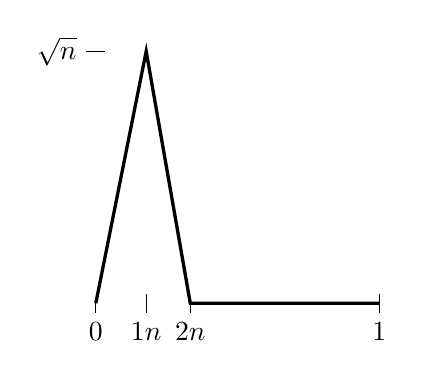
\begin{tikzpicture}[scale=0.8]
			
				\bigarrow (0,0) -- (5,0);
				\bigarrow (0,0) -- (0,5);
				
				\draw [very thick] (0,0) -- (0.8,4) -- (1.5,0) -- (4.5,0);
				
				\draw (-0.15,4) node [left] {$\sqrt{n}$} -- (0.15,4);
				\draw (0.8,-0.15) node [below] {$\f{1}{n}$} -- (0.8,0.15);
				\draw (1.5,-0.15) node [below] {$\f{2}{n}$} -- (1.5,0);

				\draw (4.5,0.15) -- (4.5,-0.15) node [below] {$1$};
				\draw (0,0) -- (0,-0.15) node [below] {$0$};
			
			\end{tikzpicture}
		\end{minipage}
		\begin{minipage}{0.53\textwidth}
			\begin{equation*}
				f_n(x) =
				\begin{cases}
					x/\sqrt{n} & \text{if } 0\leq x<1/n, \\
					2\sqrt{n} - x/\sqrt{n} & \text{if } 1/n\leq x<2/n, \\
					0 & \text{if } 2/n \leq x \leq 1.
				\end{cases}
			\end{equation*}
		\end{minipage}
	\end{center}

	Then $d_1(f_n,0)$ is the area of the triangle, while $d_\infty(f_n,0)$ is $\sqrt{n}$. Thus we have
	\begin{equation*}
		\lim_{n \to \infty} d_1(f_n,0) = 0
		\qqand
		\lim_{n \to \infty} d_\infty(f_n,0) = \infty,
	\end{equation*}
	and so these two metrics cannot possibly be Lipschitz equivalent.
\end{proof}

\begin{exercise}
	Continuing the example above, show that $d_2(f_n,0)=\sqrt{2/3}\,$ for all $n$, and so $d_2$ is not Lipschitz equivalent to $d_1$ or $d_\infty$ on $C[0,1]$.
\end{exercise}

% subsection introduction (end)

	\pagebreak

\subsection{Open balls and open sets} % (fold)
\label{sub:open_balls_and_open_sets}

\begin{definition}
	Let $(X,d)$ be a metric space, $P\in X$ and $\delta>0$. The \emph{open ball of radius $\delta$ about $p$} is given by
	\begin{equation*}
		B_d(P,\delta) := \left\{Q\in X : d(P,Q)<\delta\right\},
	\end{equation*}
	often also denoted by $B(P,\delta)$ or $B_\delta(P)$.
\end{definition}

\begin{examples}
\mbox{}
\begin{enumerate}
	\shortskip
	\item In $(\R,d_1)$, open balls are open intervals of the form $(P-\delta,P+\delta)$.
	\item In $\R^2$, we obtain different open balls depending on our choice of metric:
	\begin{itemize}
		\shortskip
		\item In $(\R^2,d_1)$, we obtain tilted squares or ``diamonds''.
		\item In $(\R^2,d_2)$, we obtain open discs of radius $\delta$.
		\item In $(\R^2,d_\infty)$, open balls are squares.
	\end{itemize}
	\mbox{}
	\begin{center}
		\begin{minipage}{0.3\textwidth}
			\centering
			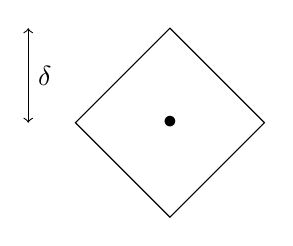
\begin{tikzpicture}[scale=1.2]
				\draw (0,-1) -- (1,0) -- (0,1) -- (-1,0) -- cycle;
				\draw (0,0) node {$\bullet$};

				\draw [<->] (-1.5,1) -- (-1.5,0);
				\draw (-1.5,0.5) node [right] {$\delta$};
			\end{tikzpicture}

			$(\R_2,d_1)$
		\end{minipage}
		\begin{minipage}{0.3\textwidth}
			\centering
			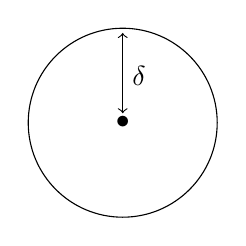
\begin{tikzpicture}[scale=1.2]
				\draw (0,0) circle (1);
				\draw (0,0) node {$\bullet$};

				\draw [<->] (0,0.95) -- (0,0.1);
				\draw (0,0.5) node [right] {$\delta$};
			\end{tikzpicture}

			$(\R_2,d_2)$
		\end{minipage}
		\begin{minipage}{0.3\textwidth}
			\centering
			\begin{tikzpicture}[scale=1.2]
				\draw (-1,-1) rectangle (1,1);
				\draw (0,0) node {$\bullet$};

				\draw [<->] (0,0.95) -- (0,0.1);
				\draw (0,0.5) node [right] {$\delta$};
			\end{tikzpicture}

			$(\R_2,d_\infty)$
		\end{minipage}
	\end{center}
	\mbox{}

	\item In $(C[0,1],d_\infty)$, the open ball of radius $\delta$ is the area swept out by translating the image of the function up and down by a distance $\delta$.
	
	\mbox{}

	\begin{center}
		\begin{tikzpicture}[scale=2,xscale=3, domain=0:1, yscale=1.2]
			\draw [->] (0,0) -- (1.2,0);
			\draw [->] (0,0) -- (0,1.8);

			\foreach \s in {0,1} {
				\draw (\s,0) -- (\s,-0.05) node [below] {$\s$};
			}

			\draw [thick] plot [smooth, id=main] function {0.05*(2*x-1)*(8*x-1)*(8*x-7)*(x-1)*(x-2)+1.1};
			\draw [dashed] plot [smooth, id=lower] function {0.05*(2*x-1)*(8*x-1)*(8*x-7)*(x-1)*(x-2)+0.8};
			\draw [dashed] plot [smooth, id=upper] function {0.05*(2*x-1)*(8*x-1)*(8*x-7)*(x-1)*(x-2)+1.4};

			\draw [<->] (1.05,1.1) -- (1.05,1.4);
			\draw (1.05,1.25) node [right] {$\delta$};
		\end{tikzpicture}
	\end{center}
	\mbox{}

	\item For any set $X$, in $(X,d_\text{disc})$, we have $B(P,\f{1}{2}) = \{P\}$ for all $P\in X$.
\end{enumerate}
\end{examples}

\begin{definition}
	A subset $U\subset X$ of a metric space $(X,d)$ is called an \emph{open subset} if, for all $P \in U$, there is some $\delta>0$ such that the open ball $B(P,\delta)$ is contained in $U$. (Note that the empty set $\emptyset$ is open, as is the whole space $X$.)

	Under this definition, an open subset is a union of (usually infinitely many) open balls.

	As the opposite to this definition, a subset $F\subset X$ is a \emph{closed subset} if $X\backslash F$ is open.
\end{definition}

\begin{example}
	Analogously to open balls, we can define \emph{closed balls}:
	\begin{equation*}
		\closure{B}(P,\delta) := \left\{Q\in X: d(P,Q) \leq \delta\right\},
	\end{equation*}
	which is the union of the open ball $B(P,\delta)$ and its boundary. The name is appropriate: these are indeed closed.

	Consider: if $Q\not\in\closure{B}(P,\delta)$, then $d(P,Q)>\delta$, and we can find $\delta\p<d(P,Q) - \delta$. Then consider a point $R \in B(Q,\delta\p)$. Then
	\begin{equation*}
		d(P,R)
		\geq d(P,Q) - d(R,Q)
		> d(P,Q) - \delta\p
		> \delta.
	\end{equation*}
	Thus $B(Q,\delta\p) \subset X\backslash\closure{B}$. Then $\closure{B}(P,\delta)$ is closed since the complment is open.
\end{example}

\begin{lemma}
\mbox{}
\begin{enumerate}
	\shortskip
	\item Both $X$ and $\emptyset$ are open subsets of $(X,d)$.
	\item If $\{U_i:i\in I\}$ are open subsets of $(X,d)$, then so is $\bigcup_{i\in I} U_i$.
	\item If $U_1,U_2$ are open subsets, then so is $U_1 \cap U_2$.
\end{enumerate}
\end{lemma}

\begin{proof}
	Both (i) and (ii) are easy, and left as exercises.
	
	For (iii): if $P \in U_1 \cap U_2$, then there are open balls $B(P,\delta_1)\subset U_1$ and $B(P,\delta_2) \subset U_2$. Thus, if $\delta=\min\{\delta_1,\delta_2\}$, then $B(P,\delta) \subset U_1 \cap U_2$. %
\end{proof}

\begin{definition}
	If $P$ is a point in $(X,d)$, then an \emph{open neighbourhood $N$ of $P$} is an open subset $N\ni P$, such as the open balls centred on $P$.
\end{definition}

\begin{example}
	Under the British Rail metric $\rho$ on $\R^2$, what are the open neighbourhoods of a point $P$? Recall that we have a point $0\in X$, %
	\begin{equation*}
		\rho(P,Q) =
		\begin{cases}
			d(P,0) + d(0,Q) & \text{if } P\neq Q, \\ %
			0 & \text{if } P=Q,
		\end{cases}
	\end{equation*}
	where $d$ is the Euclidean metric.
	
	Hence, if $P\neq 0$, $\delta<d(P,0)$, then we have $B_\rho(P,\delta) = \{P\}$. If $P=0$, $B_\rho(P,\delta)$ is an open Euclidean disc of radius $\delta$. %
	
	Thus, if $U\subset(\R^2,\rho)$ is open, then either $0\not\in U$ and $U$ is arbitrary, or $U \supseteq B_\text{eucl}(0,\delta)$ for some $\delta>0$ ($U$ contains a Euclidean disc). %
\end{example}

% subsection open_balls_and_open_sets (end)

	\pagebreak

\subsection{Limits and continuity} % (fold)
\label{sub:limits_and_continuity}

\begin{definition}
	Suppose $x_1,x_2,\ldots$ is a sequence of points in a metric space $(X,d)$. We say that $x_n$ \emph{converges to a limit} $x$ (denoted $x_n \to x$) if $d(x_n,x) \to 0$ as $n\to\infty$.
	
	Equivalently, for any $\epsilon>0$, there is some $N(\epsilon)$ such that $x_n \in B(x,\epsilon)$ for all $n\geq N$. Both of these definitions should be familiar from \emph{Analysis}. %
\end{definition}

\begin{examples}
\begin{enumerate}
	\item $1+p+p^2+\cdots+p^{n-1} \to \df{1}{1-p}$ in $(\Q,d_p)$.
	\item Consider the sequences of functions $f_n$ defined in the proof of proposition~\ref{prop:not-lip-equiv}. We have different limits, depending on our choice of metric. Clearly in $(X,d_1)$, we have $f_n \to 0$, but this is not the case in $(X,d_2)$ or $(X,d_\infty)$.
\end{enumerate}
\end{examples}

\begin{proposition}
	We have $x_n \to x$ in $(X,d)$ if and only if, for any open neighbourhood $U\ni x$, there is some $N$ such that $x_n \in U$ for all $n\geq N$.
\end{proposition}

\begin{proof}
	The ``if'' direction is clear by taking $U=B(x,\epsilon)$, for arbitrary $\epsilon$. For the converse, given an open set $U\ni x$, there is some $\epsilon>0$ such that $B(x,\epsilon) \subset U$. Hence there is some $N$ such that $x_n \in B(x,\epsilon) \subset U$ for all $n\geq N$.
\end{proof}

This allows us to rephrase $x_n \to x$ in terms of open subsets in $(X,d)$.

\begin{example}
	Take $X=C[0,1]$, $d=d_1$, and the function $g_n$ given by: %

	\begin{center}
		\begin{minipage}{0.45\textwidth}
			\centering
			\begin{tikzpicture}[scale=0.8]
			
				\bigarrow (0,0) -- (5,0);
				\bigarrow (0,0) -- (0,5);
				
				\draw [very thick] (0,4) -- (1.5,0) -- (4.5,0);
				
				\draw (-0.15,4) node [left] {$1$} -- (0.15,4);
				\draw (1.5,-0.15) node [below] {$\f{1}{n}$} -- (1.5,0);

				\draw (4.5,0.15) -- (4.5,-0.15) node [below] {$1$};
				\draw (0,0) -- (0,-0.15) node [below] {$0$};
			
			\end{tikzpicture}
		\end{minipage}
		\begin{minipage}{0.53\textwidth}
			\begin{equation*}
				g_n(x) =
				\begin{cases}
					1-nx & \text{if } 0\leq x<1/n, \\
					0 & \text{if } 1/n\leq x\leq 1.
				\end{cases}
			\end{equation*}
		\end{minipage}
	\end{center}

	Then $g_n(0)=1$ for all $n$, but $d_1(g_n,0) \to 0$; that is, $g_n \to 0$ in $(X,d_1)$ as $n\to\infty$.
\end{example}

\begin{definition}
	We say that a function $f:(X,\rho_1) \to (Y,\rho_2)$ is
	\begin{itemize}
		\shortskip
		\item \emph{continuous} at $x\in X$ if, given $\epsilon > 0$, there exists $\delta>0$ such that $\rho_1(x,x\p) < \delta$ implies $\rho_2(f(x), f(x\p))<\epsilon$ for all $x\p\in X$.
		\item \emph{uniformly continuous on $X$} if, given $\epsilon > 0$, there exists $\delta>0$ such that $\rho_1(x,x\p) < \delta$ implies $\rho_2(f(x), f(x\p))<\epsilon$ for all $x,x\p\in X$.
	\end{itemize}
\end{definition}

	\vspace{3pt}

\begin{remark}
	We may rephrase this: $f: (X,\rho_1) \to (Y,\rho_2)$ is continuous at $x\in X$ if, given $\epsilon>0$, there exists $\delta>0$ such that $f(B(x,\delta)) \subset B(f(x),\epsilon)$; that is, $B(x,\delta) \subset f^{-1}(B(f(x),\epsilon))$.
\end{remark}

	\pagebreak

\begin{lemma}
	If $f:(X,\rho_1) \to (Y,\rho_2)$ is continuous and $x_n\to x$ in $(X,\rho_1)$, then $f(x_n) \to f(x)$ in $(Y,\rho_2)$.
\end{lemma}

\begin{proof}
	Given $\epsilon>0$, there exists $\delta>0$ such that $\rho_1(x,x\p)<\delta$ implies $\rho_2(f(x),f(x\p)) < \epsilon$. As $x_n\to x$, we know there exists $N$ such that for all $n\geq N$, $\rho_1(x_n,x)<\delta$. Hence, for $n\geq N$, $\rho_2(f(x_n),f(x))<\epsilon$, and so $f(x_n) \to f(x)$.
\end{proof}

\begin{example}
	Consider the identity map $\id: (C[0,1],d_\infty) \to (C[0,1],d_1)$. Since $d_\infty(f,g) < \epsilon$ is equivalent to $\sup_{x\in [0,1]} \left\vert f(x)-g(x) \right\vert< \epsilon>$, which implies $d_1(f,g)<\epsilon$, we see that $\id$ is continuous.

	However, we can use the functions $f_n$ in the proof of proposition~\ref{prop:not-lip-equiv} to see that the identity in the opposite direction, $\id:(C[0,1], d_1) \to (C[0,1], d_\infty)$, is not continuous. We note that $d_1(f_n,0) \to0$ but $d_\infty(f_n,0) \to \infty$ as $n\to\infty$.
\end{example}

Now we wish to express continuity of maps purely in terms of open sets.

\begin{proposition}
\mbox{}
\begin{enumerate}
	\shortskip
	\item A map $f:(X,\rho_1) \to (Y,\rho_2)$ of a metric space is continuous if and only if, for any open subset $U\subset Y$, the pre-image $f^{-1}(U)$ is open in $(X,\rho_1)$.
	\item The map $f$ is continuous if and only if, for every closed subset $F\subset Y$, the pre-image $f^{-1}(F)$ is closed in $(X,\rho_1)$.
\end{enumerate}
\end{proposition}

\begin{proof}
\mbox{}
\begin{enumerate}
	\item ($\Leftarrow$) Take $U=B_{\rho_2}(f(x),\epsilon)$. If $f^{-1}(U)$ is open, then there exists $\delta>0$ such that $B_{\rho_1}(x,\delta)\subset f^{-1}(U)$; that is, $\rho_1(x',x)<\delta$ implies $\rho_2(f(x'),f(x))<\epsilon$. %
	
	($\Rightarrow$) If $U\subset Y$ is open, then consider a point $x\in f^{-1}(U)$. Since $U$ is open, we can choose a open ball $B_{\rho_2}(f(x),\epsilon)\subset U$. Since $f$ is continuous at $x$, there exists $\delta>0$ such that $B_{\rho_1}(x,\delta) \subset f^{-1}(B_{\rho_2}(f(x),\epsilon)) \subset f^{-1}(U)$. Since this is true for all $x\in f^{-1}(U)$, we have $f^{-1}(U)$ open. %
	
	\item Note that $f^{-1}(Y\backslash F)=X\backslash f^{-1}(F)$. So if $F$ is closed, then $Y\backslash F$ is open and hence $f^{-1}(Y\backslash F)$ is open. Then $X\backslash f^{-1}(F)$ is open and $f^{-1}(F)$ is closed. %
	
	Conversely, if $U$ is open in $Y$, then $Y\backslash U$ is closed in $Y$. Then $f^{-1}(Y\backslash U)=X-f^{-1}(U)$ is closed in $X$, and hence $f^{-1}(U)$ is open in $X$; that is, $f$ is continuous. \qedhere
\end{enumerate}
\end{proof}

% subsection limits_and_continuity (end)

	\pagebreak

\subsection{Completeness} % (fold)
\label{sub:completeness}

\begin{definition}
	A metric space $(X,\rho)$ is called \emph{complete} if, for any sequence $x_1,x_2,\ldots \in X$ such that, given $\epsilon>0$, there exists $N$ such that for all $m,n\geq N$, $\rho(x_m,x_n)<\epsilon$, we have $x_n\to x$ for some limit point $x$. That is, every Cauchy sequence in $X$ converges in $X$.
\end{definition}

Recall that $(\R,d_1)$ is complete; this is sometimes referred to as \emph{Cauchy's principle of convergence}. However, neither $(\Q,d_1)$ nor $((0,1) \subset \R, d_\text{Eucl})$ are complete.

\begin{example}
	Let $X=C[0,1]$ and $\rho=d_1$. This is not complete, for consider $f_n$ as shown:

	\begin{center}
		\begin{minipage}{0.45\textwidth}
			\centering
			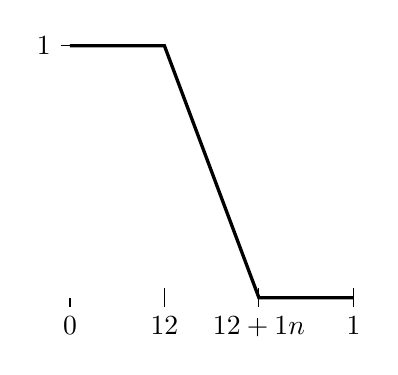
\begin{tikzpicture}[scale=0.8]
			
				\bigarrow (0,0) -- (5,0);
				\bigarrow (0,0) -- (0,5);
				
				\draw [very thick] (0,4) -- (1.5,4) -- (3,0) -- (4.5,0);
				
				\draw (-0.15,4) node [left] {$1$} -- (0.15,4);
				\draw (1.5,-0.15) node [below] {$\f{1}{2}$} -- (1.5,0.15);
				\draw (3,-0.15) node [below] {$\f{1}{2}+\f{1}{n}$} -- (3,0.15);

				\draw (4.5,0.15) -- (4.5,-0.15) node [below] {$1$};
				\draw (0,0) -- (0,-0.15) node [below] {$0$};
			
			\end{tikzpicture}
		\end{minipage}
		\begin{minipage}{0.53\textwidth}
			\begin{equation*}
				f_n(x) =
				\begin{dcases}
					1 & \text{if } 0\leq x<\tf{1}{2}, \\
					1-nx & \text{if } \tf{1}{2} \leq x <\tf{1}{2}+\tf{1}{n}, \\
					0 & \text{if } \tf{1}{2}+\tf{1}{n} \leq x \leq 1.
				\end{dcases}
			\end{equation*}
		\end{minipage}
	\end{center}

	Then for $m,n \geq N$, we have $\rho(f_m,f_n) \leq 1/N$.

	Now, if $f_n \to f \in C[0,1]$, then $\int_0^1 \left\vert f_n-f \right\vert \to f$. But
	\begin{align*}
		\int_0^1 \left\vert f_n - f \right\vert
		&\geq \int_0^{1/2} \left( \left\vert f-1 \right\vert - \left\vert f_n-1 \right\vert \right) + \int_{1/2}^1 \left( \left\vert f \right\vert-\left\vert f_n \right\vert \right) \\
		&\to \int_0^{1/2} \left\vert f-1 \right\vert + \int_{1/2}^1 \left\vert f \right\vert \geq 0.
	\end{align*}
	Thus we must have
	\begin{equation*}
		\int_0^{1/2} \left\vert f-1 \right\vert = 0
		\qqand
		\int_{1/2}^1 \left\vert f \right\vert = 0,
	\end{equation*}
	and our limit is given by
	\begin{equation*}
		f(x) =
		\begin{cases}
			1 & x\leq 1/2, \\
			0 & x>1/2,
		\end{cases}
	\end{equation*}
	but this contradicts $f \in C[0,1]$. Hence this space is not complete.
\end{example}

% subsection completeness (end)